%!TEX root = ../thesis.tex
%*******************************************************************************
%****************************** Third Chapter **********************************
%*******************************************************************************
\chapter{Complexity Conjectures} \label{chap:complexity}

% **************************** Define Graphics Path **************************
\ifpdf
    \graphicspath{{Chapter3/Figs/Raster/}{Chapter3/Figs/PDF/}{Chapter3/Figs/}}
\else
    \graphicspath{{Chapter3/Figs/Vector/}{Chapter3/Figs/}}
\fi

\section{Exponential Time Hypothesis}
Of all the algorithms covered in the previous chapter, they all had exponential computational
time complexity, with all of the backtracking based algorithms requiring $\mathcal{O}^*(2^n)$ in the worst case. Slightly better was
Sch\"oning's Algorithm \ref{alg:schoning}, which had a complexity of
$\mathcal{O}^*((2 - \frac{2}{k})^n)$. However, for a general formula in CNF
$k$ could be arbitrarily large and as $k \to \infty$ then we recover the same
complexity as the other algorithms. So even when considering the case where we
have a 3SAT instance, we are unable to improve over the
exponential complexity.

\nomenclature[x-Ostar]{$\mathcal{O}^{\ast}(\cdot)$}{Big-O ignoring polynomial factors}

We know that $k$-SAT is NP-COMPLETE for $k \geq 3$\cite{schaefer1978complexity},
so unless $P = NP$ we should not expect to find a polynomial time algorithm.
However, it is still theoretically possible, under the assumption that $P \neq NP$, for there to exist an algorithm which is superpolynomial but subexponential.
Here we say that $f(x)$ is subexponential if it is $\mathcal{O}^{\ast}(2^{\epsilon n})$ for all
$\epsilon > 0, \quad \epsilon \in \mathbb{R}$ with $\mathcal{O}^{\ast}(g(x))$ meaning $\mathcal{O}(poly(n) \cdot g(x))$,
i.e. ignoring polynomial factors. Such an algorithm
could have running time $T(n) = \mathcal{O}^{\ast}(2^{\frac{n}{\log n}})$ which is 
$\mathcal{O}^{\ast}(2^{\epsilon n}),\quad \epsilon > 0$.
However, no such algorithm for SAT has been found.

Due to the seeming difficulty of finding significantly faster $k$-SAT algorithms
there have been two conjectures
put forward by Impagliazzo and Paturi, which
relate to the complexity of $k$-SAT. These are the ``Exponential Time Hypothesis'' and the ``Strong
Exponential Time Hypothesis'', abbreviated to ETH and SETH respectively \cite{impagliazzo2001complexity}.

\nomenclature[z-ETH]{ETH}{Exponential Time Hypothesis}
\nomenclature[z-SETH]{SETH}{Strong Exponential Time Hypothesis}

Informally ETH hypothesises that there does not exist a subexponential time algorithm solving SAT.
More formally, consider the set of all $k$-SAT algorithms and
express their time complexities in the form $\mathcal{O}^{\ast}(2^{\delta n})$
for some constant $\delta \in \mathbb{R}^{+} \cup \{0\}$.
Then for $k \in \mathbb{N}, \quad k \geq 3$ let $s_k$ be the infimum
of $\delta$s taken from this set
\begin{equation} \label{eq:ETH}
    s_k = \inf \{\delta: \text{$k$-SAT is solvable in time } \mathcal{O}^{\ast}(2^{\delta n})\}
\end{equation}
The ETH then states that $s_{3} > 0$ \cite{impagliazzo2001complexity}.
Intuitively this means that there must exist some non-zero constant $s_{3}$ such
that solving 3-SAT takes time $\Omega^{\ast}(2^{s_{3} n})$ which rules out
a subexponential time algorithm for 3-SAT.
The statement that $s_3 > 0$ is equivalent to the statement that
for all $k \in \mathbb{N}$ if $k \geq 3$ then $s_k > 0$,
i.e. there then cannot exist a subexponential time
algorithm for $k$-SAT with $k \geq 3$. This is because a 3-CNF can be easily
reduced to a $k$-CNF for all $k \geq 3$.

If we, instead of considering all $k$-SAT algorithms, consider just Sch\"oning's
algorithm, then we get a new sequence of $s'_k$ where 
$\forall k \in \mathbb{N}: s'_k \geq s_k$. Rearranging the complexity
of Sch\"oning's algorithm we get that

\begin{equation} \label{eq:sk_schoing}
    s'_k = \log_2(2 - \frac{2}{k}), \quad k \geq 3
\end{equation}

which yields the sequence $\sim 0.415, \sim 0.585, \sim 0.678, \dots$ for
$k= 3,4,5, \dots$. It is clear from Equation \ref{eq:sk_schoing} that
as $k \to \infty$ then $s'_k \to 1$.
There are known algorithms that produce smaller constants \cite{hofmeister2002probabilistic},
however these algorithms still generate a sequence that tends to 1 as
$k \to \infty$.

The ``Strong Exponential Time Hypothesis'' (SETH) considers this limit
as $k$ tends to infinity. SETH states that
\begin{equation} \label{eq:SETH}
    \lim_{k \to \infty} s_{k} = 1
\end{equation}
Intuitively, if SETH were proven true,
this would mean that for general SAT there is no algorithm that is
asymptotically faster than brute force search and algorithms
such as DP, DPLL and CDCL would be optimal up to subexponential factors.
% highlight any differences between the formalism and the intuition

\subsection{Conditional Lower Bounds}
The ETH and SETH both imply that $P \neq NP$, so we should not hope to
prove either conjecture just yet. However, we can consider the implications
that these conjectures would have on other problems if they were proven true.
This allows for us to show that many problems have conditional lower bounds
on their complexity and for many problems that current algorithms
are optimal assuming one of these conjectures.

If we consider attempting to show lower bounds from an assumption of the ETH,
then since the ETH deals with the non-existence of subexponential time algorithms
for $k$-SAT, we could hope to reduce $k$-SAT to a number of different problems in
such a way that preserves subexponential time.

Since we are dealing with parameterized complexities for $k$-SAT with parameters
$n$ and $m$, when considering general problems we will use the mapping
$\kappa: \Sigma^* \mapsto \mathbb{N}$ to denote the parameter an instance
of the problem $x \in \Sigma^*$. Where $\Sigma^*$ is the set of problem instances.

\begin{definition}
    A Turing reduction from a problem $(A_1, \kappa_1)$ to a problem
    $(A_2, \kappa_2)$ is considered a SERF-T reduction if
    \begin{enumerate}
        \item The reduction on an instance $x$ of $A_1$
        runs in time $\mathcal{O}(2^{\epsilon \kappa_1(x)}|x|^{\mathcal{O}(1)})$
        for a choice of $\epsilon > 0$.
        \item For a query to $A_2$ with input $x'$:
        \begin{enumerate}
            \item $|x'| \leq |x|^{\mathcal{O}(1)}$
            \item $\kappa_2(x') \leq \alpha \kappa_1(x)$
        \end{enumerate}
        Where the constants hidden in the $\mathcal{O}(\cdot)$ do not
        depend on the choice of $\epsilon$.
        The constant $\alpha$ may depend on $\epsilon$
    \end{enumerate}
\end{definition}

To see how this works, consider two parameterized problems $(A_1, \kappa_1)$
and $(A_2, \kappa_2)$, where the second problem has a parameterized
subexponential time algorithm. We wish to show that if $(A_1, \kappa_1)$ is
SERF-T reducible to $(A_2, \kappa_2)$ then there also exists a parameterized
subexponential time algorithm for $(A_1, \kappa_1)$, i.e. for a choice of
$\epsilon > 0$ we need to show that $(A_1, \kappa_1)$ runs in time
$\mathcal{O}(2^{\epsilon \kappa_1(x)}|x|^{\mathcal{O}(1)})$.

Do show this, choose an $\epsilon > 0$.
Let $\epsilon' = \frac{\epsilon}{2}$ and run the SERF-T reduction
with parameter $\epsilon'$. Since this reduction runs in time
$\mathcal{O}(2^{\epsilon' \kappa_1(x)}|x|^{\mathcal{O}(1)})$ then this bounds
the number of calls to $(A_2, \kappa_2)$ by the same amount.
Each call to $(A_2, \kappa_2)$ has an instance $|x'| \leq |x|^{\mathcal{O}(1)}$
and $\kappa_2(x') \leq \alpha \kappa_1(x)$.
Since, from our assumption that $(A_2, \kappa_2)$ runs in parameterized subexponential
time we can choose $\epsilon'' = \frac{\epsilon'}{\alpha}$ and then each call to $(A_2, \kappa_2)$ can be made to run in time 
\begin{equation}
    \mathcal{O}(2^{\epsilon' \kappa_1(x)}|x|^{\mathcal{O}(1)})
\end{equation}
Therefore, the total time for solving $(A_1, \kappa_1)$ is given by
\begin{equation}
    \mathcal{O}(2^{\epsilon' \kappa_1(x)}|x|^{\mathcal{O}(1)}) \cdot
    \mathcal{O}(2^{\epsilon' \kappa_1(x)}|x|^{\mathcal{O}(1)}) =
    \mathcal{O}(2^{\epsilon \kappa_1(x)}|x|^{\mathcal{O}(1)})
\end{equation}
which is what we wanted to show. \cite{lokshtanov2013lower}

\subsubsection{Lower Bounds for 3-colouring}

To show that ETH implies that there is no subexponential time algorithm for 3-colourability
we must show that the standard reduction from 3-SAT to 3-colourability is also
a SERF-T reduction. The first requirement that the reduction runs in time 
$\mathcal{O}(2^{\epsilon \kappa_1(x)}|x|^{\mathcal{O}(1)})$ for all $\epsilon > 0$ is trivially
satisfied since the reduction runs in polynomial time.
Hence it also follows that the reduced instance $|x'| \leq |x|^{\mathcal{O}(1)}$.

Thus, the only thing left to show is that $\kappa_2(x') \leq \alpha \kappa_1(x)$ for
some constant $\alpha$. In this case $\kappa_2(x')$ would be the number of vertices
in the reduced instance and $\kappa_1(x) = n$.

To do this, recall the the standard reduction reduction from 3-SAT to 3-colourability
(see Figure \ref{fig:reduce_3col}).
We have a triangle and label the vertices as True, False and Base.
For each variable $x_i$ we create vertices labelled $x_i$ and $\neg x_i$ and
edges $(x_i, \neg x_i), (x_i, \text{Base}), (\neg x_i, \text{Base})$. Then
for each clause we have two ``or'' gadgets that consist of 3 vertices.
Thus, the total number of vertices in the instance $x'$ is given by
\begin{equation}
    \kappa_2(x') = 2n + 3m + 3
\end{equation}
This appears to be an issue, since we are unable to make $\kappa_2(x')$ linear in $n$
since $m$ could be a superlinear function of $n$ for an arbitrary instance of 3-SAT $x$.
However, we can make use of the sparsification lemma \cite{impagliazzo2001problems} to
reduce any $k$-SAT instance into a subexponential number of $k$-SAT instances where
$m$ is linear in $n$ and this takes subexponential time. We will detail the
sparsification lemma in Chapter \ref{chap:sparsication}.

Hence, to get our SERF-T reduction we first apply the sparsification lemma to
reduce our original instance $x$ into subexponentially many new $k$-SAT instances
and apply our standard 3-SAT to 3-colourability reduction to each new instance.
Since we can now guarantee that $m$ is $\mathcal{O}(n)$ then $2n + 3m + 3$ is also
$\mathcal{O}(n)$. We let $\alpha$ be the constant hidden in the $\mathcal{O}(\cdot)$.
Since the sparsification lemma produces a subexponential number of instances that
are no longer than the original instance and since it runs in subexponential time, then
we do not violate the time constraints of the SERF-T reduction.

Hence we have shown that this reduction satisfies all the requirements of a SERF-T
requirement. We can therefore say that if 3-colourability on $|V|$ vertices can
be solved in time $\mathcal{O}^{\ast}(2^{\epsilon \cdot |V|})$ for all $\epsilon > 0$
then 3-SAT could be solved in time $\mathcal{O}^{\ast}(2^{\epsilon \cdot n})$ 
for all $\epsilon > 0$, which would violate the ETH.

\begin{figure}
    \centering
    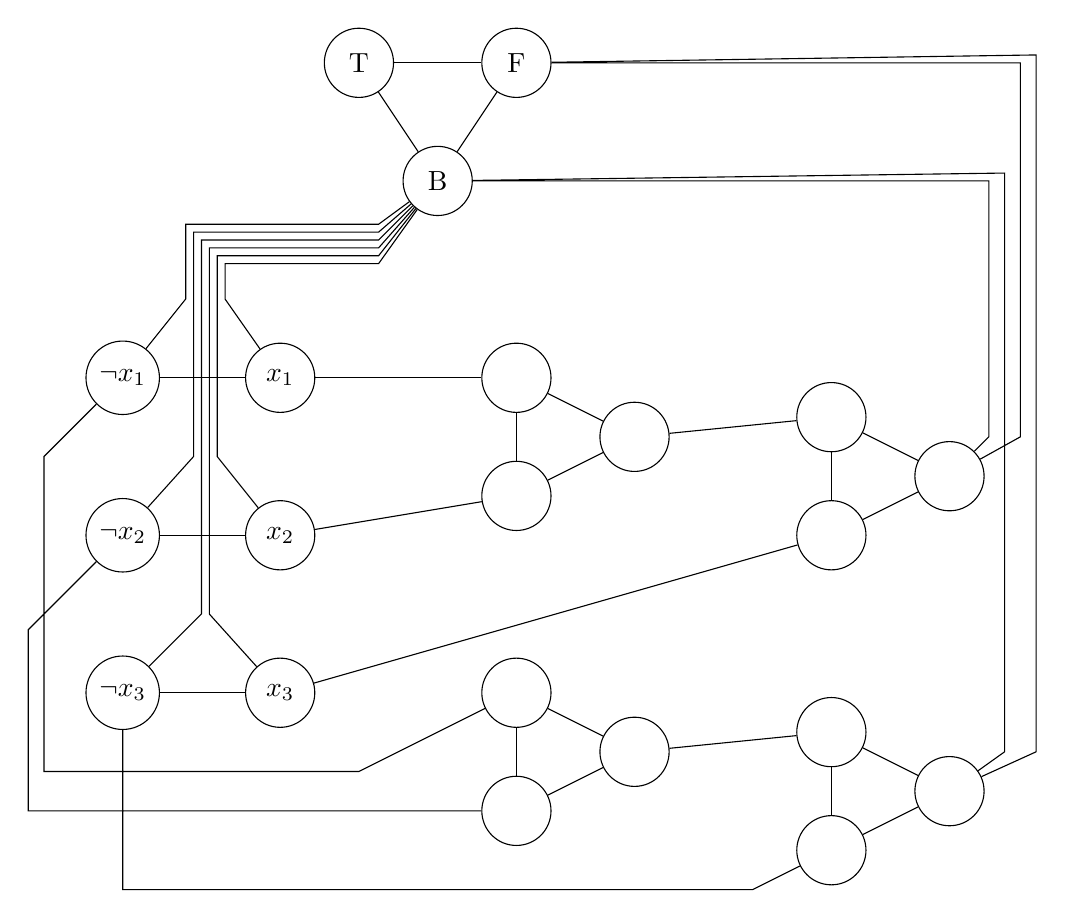
\begin{tikzpicture}
        \begin{scope}[auto,every node/.style={draw,circle,minimum size=2.5em}]
        % Pallet
        \node (T) at (-1,0) {T};
        \node (F) at (1,0) {F};
        \node (B) at (0,-1.5) {B};
        
        % Variables
        \node (x1) at (-2, -4) {$x_1$};
        \node (!x1) at (-4, -4) {$\neg x_1$};
        \node (x2) at (-2, -6) {$x_2$};
        \node (!x2) at (-4, -6) {$\neg x_2$};
        \node (x3) at (-2, -8) {$x_3$};
        \node (!x3) at (-4, -8) {$\neg x_3$};
        
        % Or gadets
        \node (or1a) at (1, -4) {};
        \node (or1b) at (2.5, -4.75) {};
        \node (or1c) at (1, -5.5) {};
        
        \node (or2a) at (5, -4.5) {};
        \node (or2b) at (6.5, -5.25) {};
        \node (or2c) at (5, -6) {};
        
        \node (or3a) at (1, -8) {};
        \node (or3b) at (2.5, -8.75) {};
        \node (or3c) at (1, -9.5) {};
        
        \node (or4a) at (5, -8.5) {};
        \node (or4b) at (6.5, -9.25) {};
        \node (or4c) at (5, -10) {};
        \end{scope}
        
        \path (T) edge (F) edge (B)
              (B) edge (F)
              (!x1) edge (x1)
              (!x2) edge (x2)
              (!x3) edge (x3)
              (or1a) edge (or1b)
              (or1b) edge (or1c)
              (or1c) edge (or1a)
              (or2a) edge (or2b)
              (or2b) edge (or2c)
              (or2c) edge (or2a)
              (or3a) edge (or3b)
              (or3b) edge (or3c)
              (or3c) edge (or3a)
              (or4a) edge (or4b)
              (or4b) edge (or4c)
              (or4c) edge (or4a)
              (x1) edge (or1a)
              (x2) edge (or1c)
              (or1b) edge (or2a)
              (x3) edge (or2c);
              
        \draw (!x1) -- (-5, -5) -- (-5 , -9) -- (-1, -9) -- (or3a)
              (!x2) -- (-5.2, -7.2) -- (-5.2, -9.5) -- (or3c)
              (or3b) -- (or4a)
              (!x3) -- (-4, -10.5) -- (4, -10.5) -- (or4c)
              (or2b) -- (7, -4.75) -- (7, -1.5) -- (B)
              (or2b) -- (7.4, -4.75) -- (7.4, 0) -- (F)
              (or4b) -- (7.2, -8.75) -- (7.2, -1.4) -- (B)
              (or4b) -- (7.6, -8.75) -- (7.6, 0.1) -- (F)
              (B) -- (-0.75, -2.25) -- (-3, -2.25) -- (-3, -7) -- (!x3)
              (B) -- (-0.75, -2.35) -- (-2.9, -2.35) -- (-2.9, -7) -- (x3)
              (B) -- (-0.75, -2.15) -- (-3.1, -2.15) -- (-3.1, -5) -- (!x2)
              (B) -- (-0.75, -2.45) -- (-2.8, -2.45) -- (-2.8, -5) -- (x2)
              (B) -- (-0.75, -2.05) -- (-3.2, -2.05) -- (-3.2, -3) -- (!x1)
              (B) -- (-0.75, -2.55) -- (-2.7, -2.55) -- (-2.7, -3) -- (x1);
        
    \end{tikzpicture}
    \caption[Reduction to 3-colourability]{Standard reduction of 
    $(x_1 \lor x_2 \lor x_3) \land (\neg x_1 \lor \neg x_2 \lor \neg x_3)$ to 3-colourability}
    \label{fig:reduce_3col}
\end{figure}

Using similar techniques we can also establish that the ETH implies that
there are no subexponential time algorithms for the following \cite{lokshtanov2013lower}.
\begin{itemize}
    \item Independent Set
    \item Dominating Set
    \item Vertex Cover
    \item Hamiltonian Path
\end{itemize}

\subsubsection{Lower Bounds for Planar Graph Problems}
Note that the SERF-T reduction from 3-SAT to 3-colourability depended on the
fact that the number of vertices in the
3-colourability instance was linear in the in the number of variables
in the 3-SAT instance. Typically for planar graph problems, this
property cannot be obtained.

For instance the reduction from 3-SAT to planar hamiltonian cycle 
creates a graph $G$ where the number of vertices is $\mathcal{O}(m^2)$ \cite{garey1976planar}.
As such we cannot establish a SERF-T reduction from 3-SAT to planar hamiltonian cycle 
parameterized by the number of vertices.
However, if we let the parameter be $\kappa_2(x') = \sqrt{|V|}$, then it is obvious that
this parameter is $\mathcal{O}(m)$. Then we can use the same techniques as before to
establish that the ETH implies that there is no $2^{o(\sqrt{|V|})}$ algorithm for planar
hamiltonian cycle.

The same argument can be made for many planar graph problems. Taken in conjunction
with algorithms using the planar separator theorem \cite{lipton1979separator} this
then means that many planar graph algorithms are optimal \cite{lipton1977applications}.

\subsection{Further Conditional Lower Bounds for Algorithms in P}
Proofs of conditional lower bounds are not limited to problems that
have superpolynomial complexities. Here we will give an example
of a lower bound for the orthogonal vectors problem based on the assumption
of the SETH \cite{williams2004new}.

\begin{definition}
    The orthogonal vectors problem is, given two sets $U$ and $V$ of bit vectors of length
    $d$ where $|U| = |V| = n$ and $d$ is $\omega(\log n)$, does there exist $u \in U$ and
    $v \in V$ such that $\sum_{i = 1}^{d} u_i \cdot v_i = 0$
\end{definition}

Best known algorithms for orthogonal vectors take time $\mathcal{O}(n^{2 - o(1)})$ and
it is unknown whether there is any ``strongly subquadratic'' algorithm, i.e. an
algorithm taking time $\mathcal{O}(n^{2 - \epsilon})$ for some $\epsilon > 0$. However,
Williams et al. show that SETH implies that no such algorithm exists \cite{williams2004new}.

To show this we will need the concept a fine grained reduction. Such a reduction
has the property that for two problems $A$ and $B$ with best known running times
$a(n)$ and $b(n)$ respectively, an improvement on $B$ to $\mathcal{O}(b(n)^{1 - \epsilon})$
leads to an improvement on $A$ to $\mathcal{O}(a(n)^{1 - \delta})$ for all $\epsilon > 0$
and some $\delta > 0$. Such a reduction is often denoted as a $(a(n), b(n))$-reduction \cite{vassilevska2015hardness}

\begin{definition}
    A fine grained reduction $M$ from problem $A$ to problem $B$ with running times
    $a(n)$ and $b(n)$ respectively obeys the following:
    For all $\epsilon > 0$, there is some $\delta > 0$ and some constant $d$
    such that for all $n \geq 1$ there is some constant $k_n$ and
    \begin{itemize}
        \item $M$ runs in time $d \cdot (a(n))^{1 - \delta}$,
        \item $M$ produces at most $k_n$ instances of $B$ adaptively,
        \item $\sum_{i = 1}^{k_n}(b(n'_i)^{1 - \epsilon}) \leq d \cdot (a(n))^{1 - \delta}$, where $n'_i$ is the
        $i_{\text{th}}$ instance of $B$. 
    \end{itemize}
    Instance sizes $n'_i$ may depend on $n$ and $\epsilon$, but $d$ can depend only on $\epsilon$ and not on $n$.
\end{definition}

The $(2^n, n^2)$-reduction from $k$-SAT to orthogonal vectors is then as follows. Apply the sparsification lemma
to the $k$-SAT instance, then partition the variables arbitrarily into two sets $D_1, D_2$ such
that each set contains $\frac{n}{2}$ variables. Construct two sets of vectors $U_1, U_2$ as follows:
For all $i \in \{1,2\}$ and for all assignments $\alpha$ to the variables in $D_i$, $v_{i, \alpha} \in U_i$
where for all clauses $C$, $v_{i, \alpha}[C] = 0$ if and only if the clause $C$ is satisfied by the
assignment $\alpha$ to the variables in $D_i$, $1$ otherwise. Therefore, if two vectors are orthogonal then
there exists an assignment to the variables in $D_1$ and $D_2$ such that for every clause it
is either satisfied by the assignment to $D_1$ or the assignment to $D_2$ \cite{williams2004new}.

Hence, any $\mathcal{O}(n^{2 - \epsilon})$ time algorithm for orthogonal vectors implies that there
is a $\mathcal{O}(2^{(1 - \delta)n})$ algorithm for $k$-SAT for all $k$. Therefore, the SETH
implies that there cannot be such an algorithm for orthogonal vectors.

Applying similar techniques, SETH implies
\begin{itemize}
    \item Fr\'echet distance cannot be computed in $\mathcal{O}(n^{2 - \epsilon})$ \cite{bringmann2014walking}
    \item Edit distance cannot be computed in $\mathcal{O}(n^{2 - \epsilon})$ \cite{backurs2015edit}
    \item Dynamic Time Warping distance cannot be computed in $\mathcal{O}(n^{2 - \epsilon})$ \cite{bringmann2015quadratic}
    \item Longest Common Subsequence cannot be computed in $\mathcal{O}(n^{2 - \epsilon})$ \cite{bringmann2018multivariate, polak2018hard}
\end{itemize}